\chapter{Compact Muon Solenoid} % Main chapter title

\label{Chapter4} % Change X to a consecutive number; for referencing this chapter elsewhere, use \ref{ChapterX}

\lhead{Chapter 4. \emph{Compact Muon Solenoid}} % Change X to a consecutive number; this is for the header on each page - perhaps a shortened title

Compact Muon Solenoid is a general purpose detector designed to be able to cover a wide range of physics at the LHC. It has a layered design with each layer detecting different kinds of particles and covering a large portion or the spherical angle around the interaction point. Inside a large soleonid, with a tracker and calorimeter built inside to improve the resolution of the momentum measurements. Detectors outside the solenoid are designed primarily to detect muons.  \\

DODATI JOS OPCENITO O CMS-u

\begin{figure}[htbp]
	\centering
		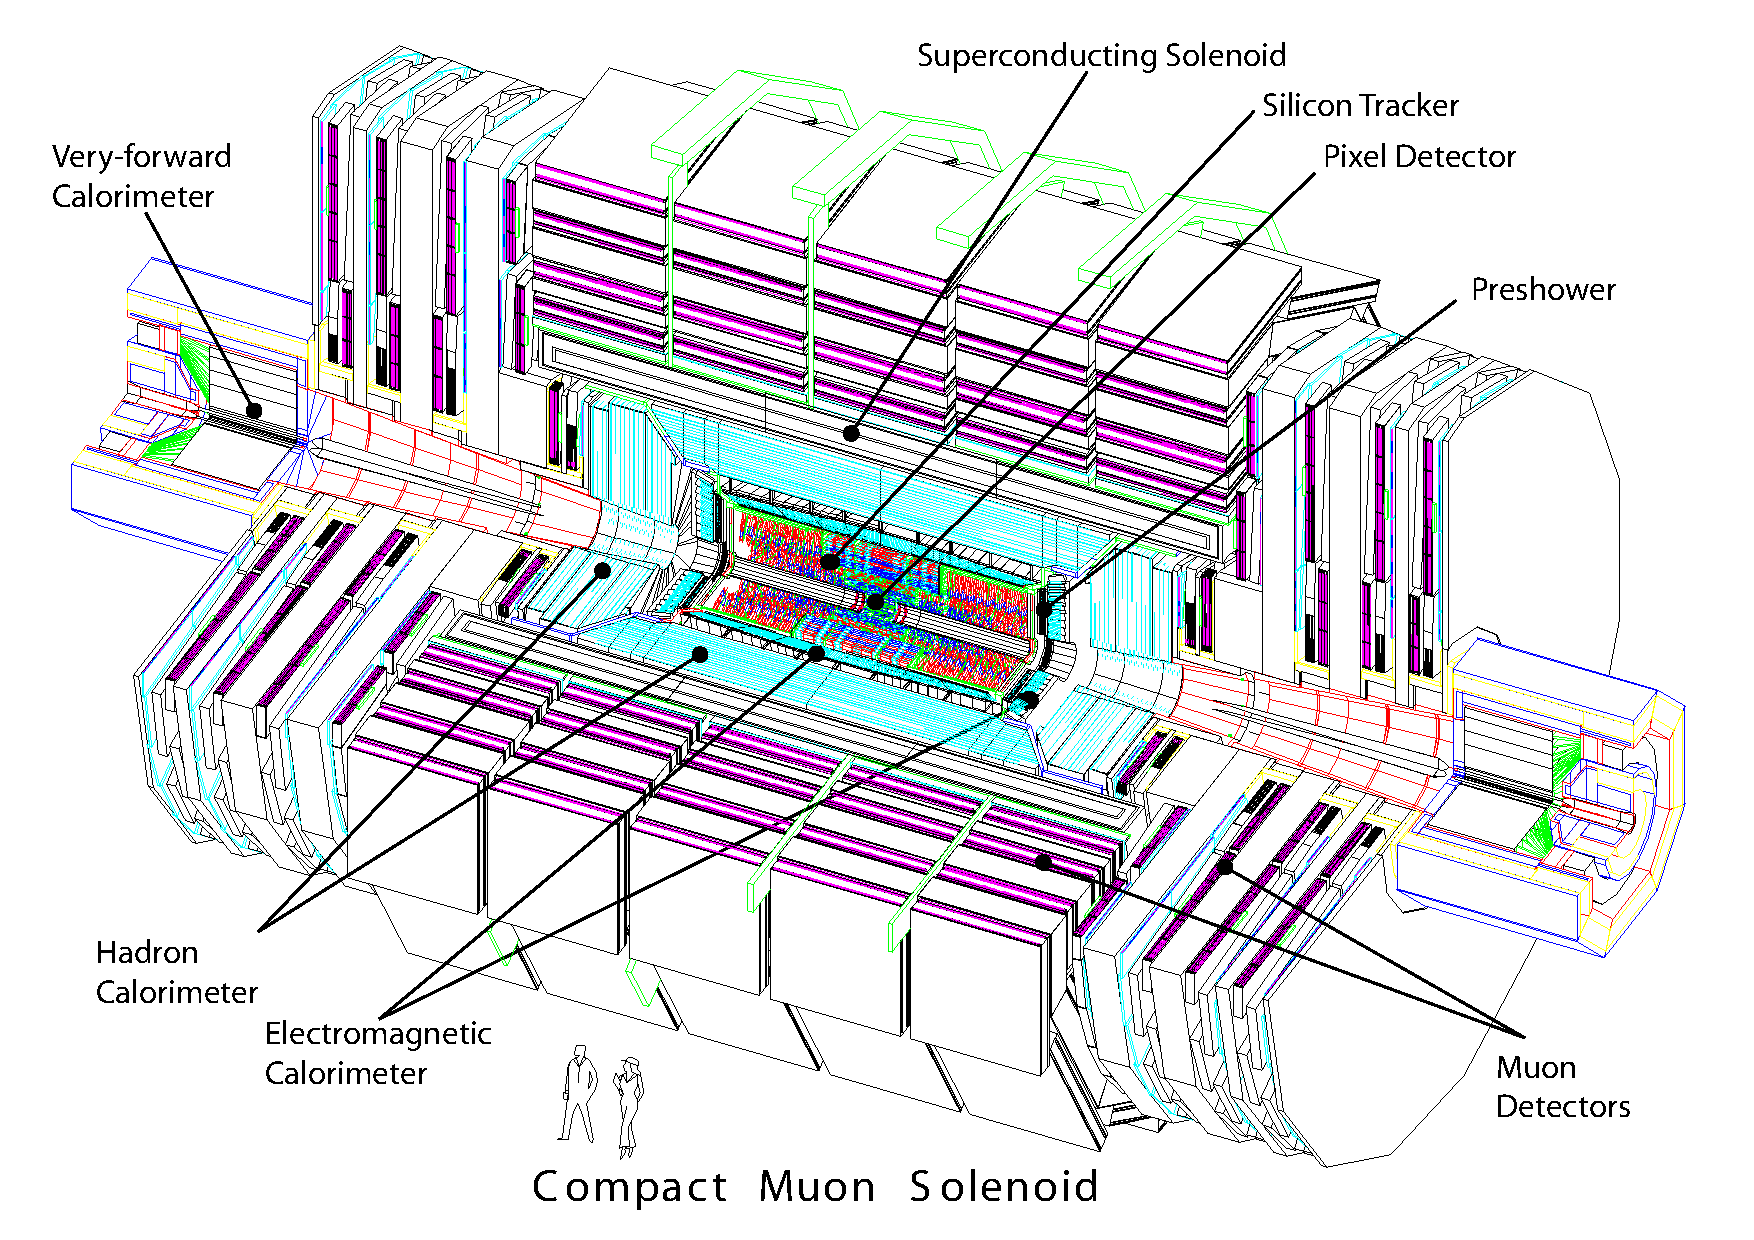
\includegraphics[width=0.8\textwidth]{Figures/CMS.pdf}
		%\rule{35em}{0.5pt}
	\caption[CMS detector]{A drawing of the CMS detector. \cite{Chatrchyan:2008aa}}
	\label{fig:CMS}
\end{figure}
\par The goals for the CMS with respect to its purpose in the LHC programme is very good muon identification and good momentum resolution over wide range of phase space and ambiguous determination of muon charge. Very good inner tracking system for detection of charged particles and high efficiency offline b quark tagging and $\tau$ tagging. Other important requirements, specially for Higgs searches, is diphoton mass resolution, and photon and electron identification and isolation at high energies. 
CMS detector with its design meets all these requirements as it shown in following sections of this chapter.  Each section describing a part of the detector separately together with it's role in CMS.  

%----------------------------------------------------------------------------------------
%	SECTION 0
%----------------------------------------------------------------------------------------

\section{CMS coordinate system}

CMS uses a right-handed coordinate system with the origin in the interaction point. $z-$axis is pointing along the beam line. $x-$axis is pointing towards the center of the ring while y axis points upwards. Two angles are used when describing position inside the detector, azimuthal angle $\phi$ and polar angle $\theta$. $\phi$ angle lies in $x-y$ plane with a range $[-\pi,\pi]$  and is defined as $\phi=$atctan$(y/x)$. The other angle $\theta$ is usually not used in high-energy physics because differences in $\theta$ are not Lorentz invariant.
The variable that is Lorentz invariant is rapidity:
\begin{equation}
y=\frac{1}{2}ln\left[ \frac{E+p_z}{E-p_z}\right]
\end{equation}
In high energy experiments in the relativistic limit where $E>>m$, a quantity called pseudorapidity is a good approximation of rapidity:
\begin{equation}
\eta = -ln \left[ tan \frac{\theta}{2} \right]
\end{equation}
Pseudorapidity Lorentz invariance means that a measurement of $\Delta\eta$ between particles is not dependent on specifying a reference frame, such as the rest frame of a particle or the laboratory frame. When using the term "forward" direction, it refers to regions of the detector that are close to the beam axis, at high |$\eta$|. When the distinction between "forward" and "backward" is relevant, the former refers to the positive z-direction and the latter to the negative z-direction.

%----------------------------------------------------------------------------------------
%	SECTION 1
%----------------------------------------------------------------------------------------

\section{Solenoid magnet}

Solenoid magnet within the CMS has the length of 12.9 m, an inner diameter of 5.9 m provides provides a magnetic field of 3.8 T. The solenoid is large enough to contain inner tracking system and calorimeters inside which reduces the material budget before the energy measurement in the calorimeters. The strong magnetic field increases the curvature of the trajectories of the highly energetic particles thus improving the momentum resolution.
\par Superconducting materials are used to build the solenoid with the operational temperature of 4.6 K. It is composed of four layers of superconducting material inserted in aluminum. Muon detectors outside the solenoid operate in 2 T magnetic field enhanced by the 10 000-t iron yoke.  

%----------------------------------------------------------------------------------------
%	SECTION 2
%----------------------------------------------------------------------------------------

\section{Inner tracker system}

The role of inner tracking system in CMS is to provide a precise measurement of charged particles trajectories created in collisions with $p_T>1$ GeV and the pseudorapidity $|\eta|<2.5$. Other important task is precise secondary vertex positions reconstruction and impact parameter determination. The size of CMS inner tracker is 5.8 m in length with a diameter of 2.5 m. Large magnetic field of 4 T is provided by the surrounding solenoid and is homogeneous across the entire inner tracking system. With the design LHC luminosity, expected occupancy of inner tracking system is more than 1000 particles from 20 primary interactions in each bunch crossing. This requires high granularity detectors with fast responses and low dead time of the detector. Trying to design a detector with these characteristics while at the same time reducing the amount of material in the detector to minimum and taking into account the radiation hardness, lead to the solution of building an all-silicon detector. CMS inner tracking system has two separate parts, Pixel detector and Strip detector which are described below.    


%-----------------------------------
%	SUBSECTION 2.1
%-----------------------------------
\subsection{Pixel Detector}

Pixel detector is the closest part of the CMS to the interaction point. Barrel pixel is the central part with three layers located at radii of 4.4 cm, 7.3 cm and 11 cm. On each side of the barrel pixel, there are two discs at $z=$ 34.5 cm and 46.5 cm. The detector is fully modular hybrid detector with silicon layer bump bonded to read-out chips where each pixel is read out separately. 

\begin{figure}[htbp]
	\centering
		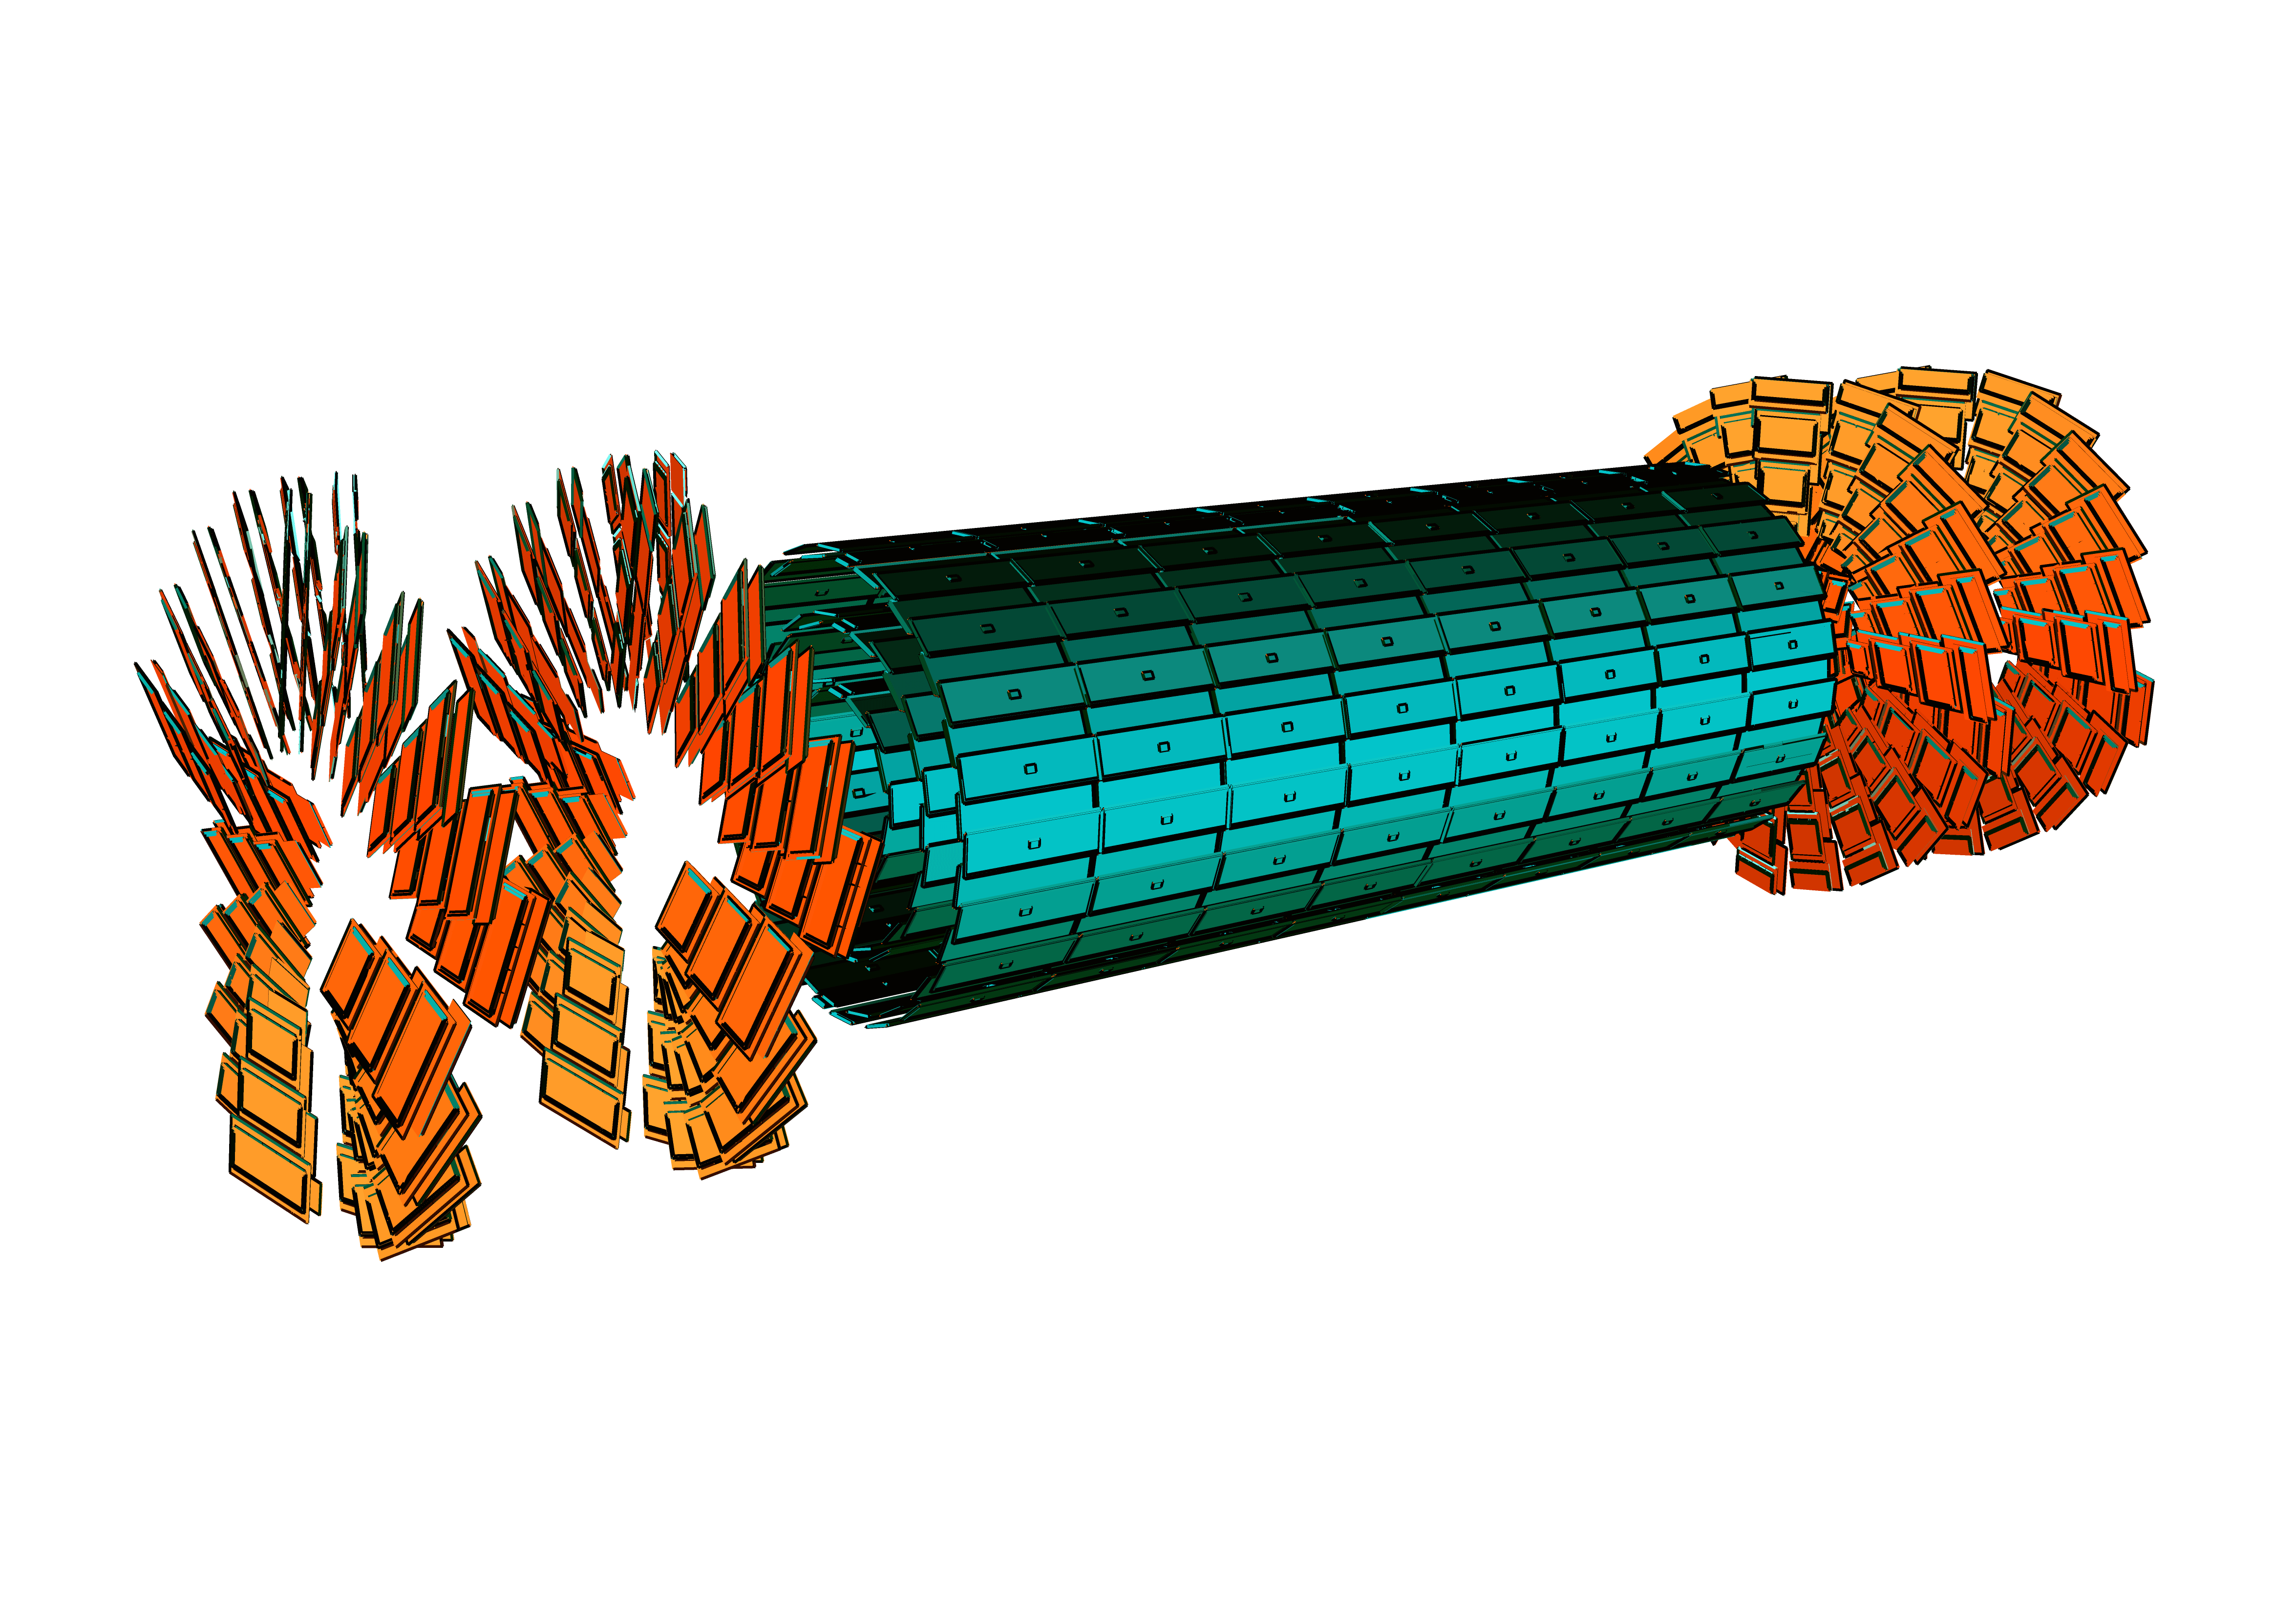
\includegraphics[width=0.8\textwidth]{Figures/pixel_detector.png}
		%\rule{35em}{0.5pt}
	\caption[CMS Pixel Detector]{A drawing of the CMS pixel detector. \cite{Chatrchyan:2008aa}}
	\label{fig:pixels}
\end{figure}
DODATI JOS O PIXELU

%-----------------------------------
%	SUBSECTION 2.2
%-----------------------------------

\subsection{Strip detector}

Silicon pixel tracker is built in layers around Pixel detector where track particle flux is lower and lower granularity detector can be used instead. Detector is built of strips in which a passing charged particle induces current. Current is than transferred to silicon detectors connected to the wires. The barrel section of the strip detector consists of four layers in the inner part (TIB) and 6 layer in the outer part (TOB). In the forward regions there are three tracker inner discs (TID) on each side of the barrel and 9 layers in the tracker endcap (TEC). 
\\par Some strips are built in double layers tilted against each other by an angle of 100 mrad to precisely measure the position of both $r\phi$ and $rz$ directions. The pitch size between strips varies from 80 $\mu m$ in the TIB to 184 $\mu$m in TOB and TEC. With the increasing distance from the interaction point, both strip pitch and strip length increase and sensor thickness becomes larger which affects the resolution.    

\begin{figure}[htbp]
	\centering
		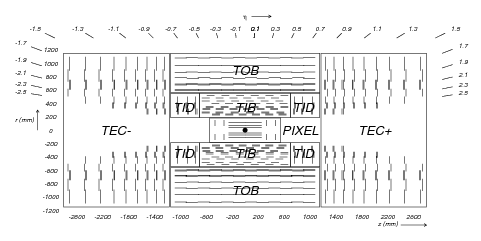
\includegraphics[width=0.8\textwidth]{Figures/strip_detector.png}
		%\rule{35em}{0.5pt}
	\caption[CMS Strip Detector]{A drawing of the CMS strip detector. \cite{Chatrchyan:2008aa}}
	\label{fig:strips}
\end{figure}

%----------------------------------------------------------------------------------------
%	SECTION 3
%----------------------------------------------------------------------------------------

\section{Electromagnetic calorimeter}

The role of the Electromagnetic calorimeter in CMS is precise measurement of electron and photon energies and corresponding electromagnetic showers. It is built from lead tungstate (PbWO$_4$), a material with very high density (8.28 g$/$cm$^3$) and a small Moliere radius (0.89 cm) which is a scale of transverse dimension of the fully contained electromagnetic showers. The scintillation light emitted within a single bunch crossing of 25 ns is about 80$\%$ of the total light which is a large advantage of this material. The calorimeters is built of 61 200 crystals in the barrel region and 14 670 crystals in the endcaps. Each crystal has a size of 22$\times $22 mm$^2$ in the front, 26$\times$26 mm$^2$ at the back side and length on 23 cm in the barrel region. In the endcaps, the size of the crystals goes from $28.62\times 28.62$ in the front to $30\times 30$ mm$^2$ in the back with a length of 22 cm. The whole systems covers the $\eta$ range to $|\eta|<3$.
\begin{figure}[htbp]
	\centering
		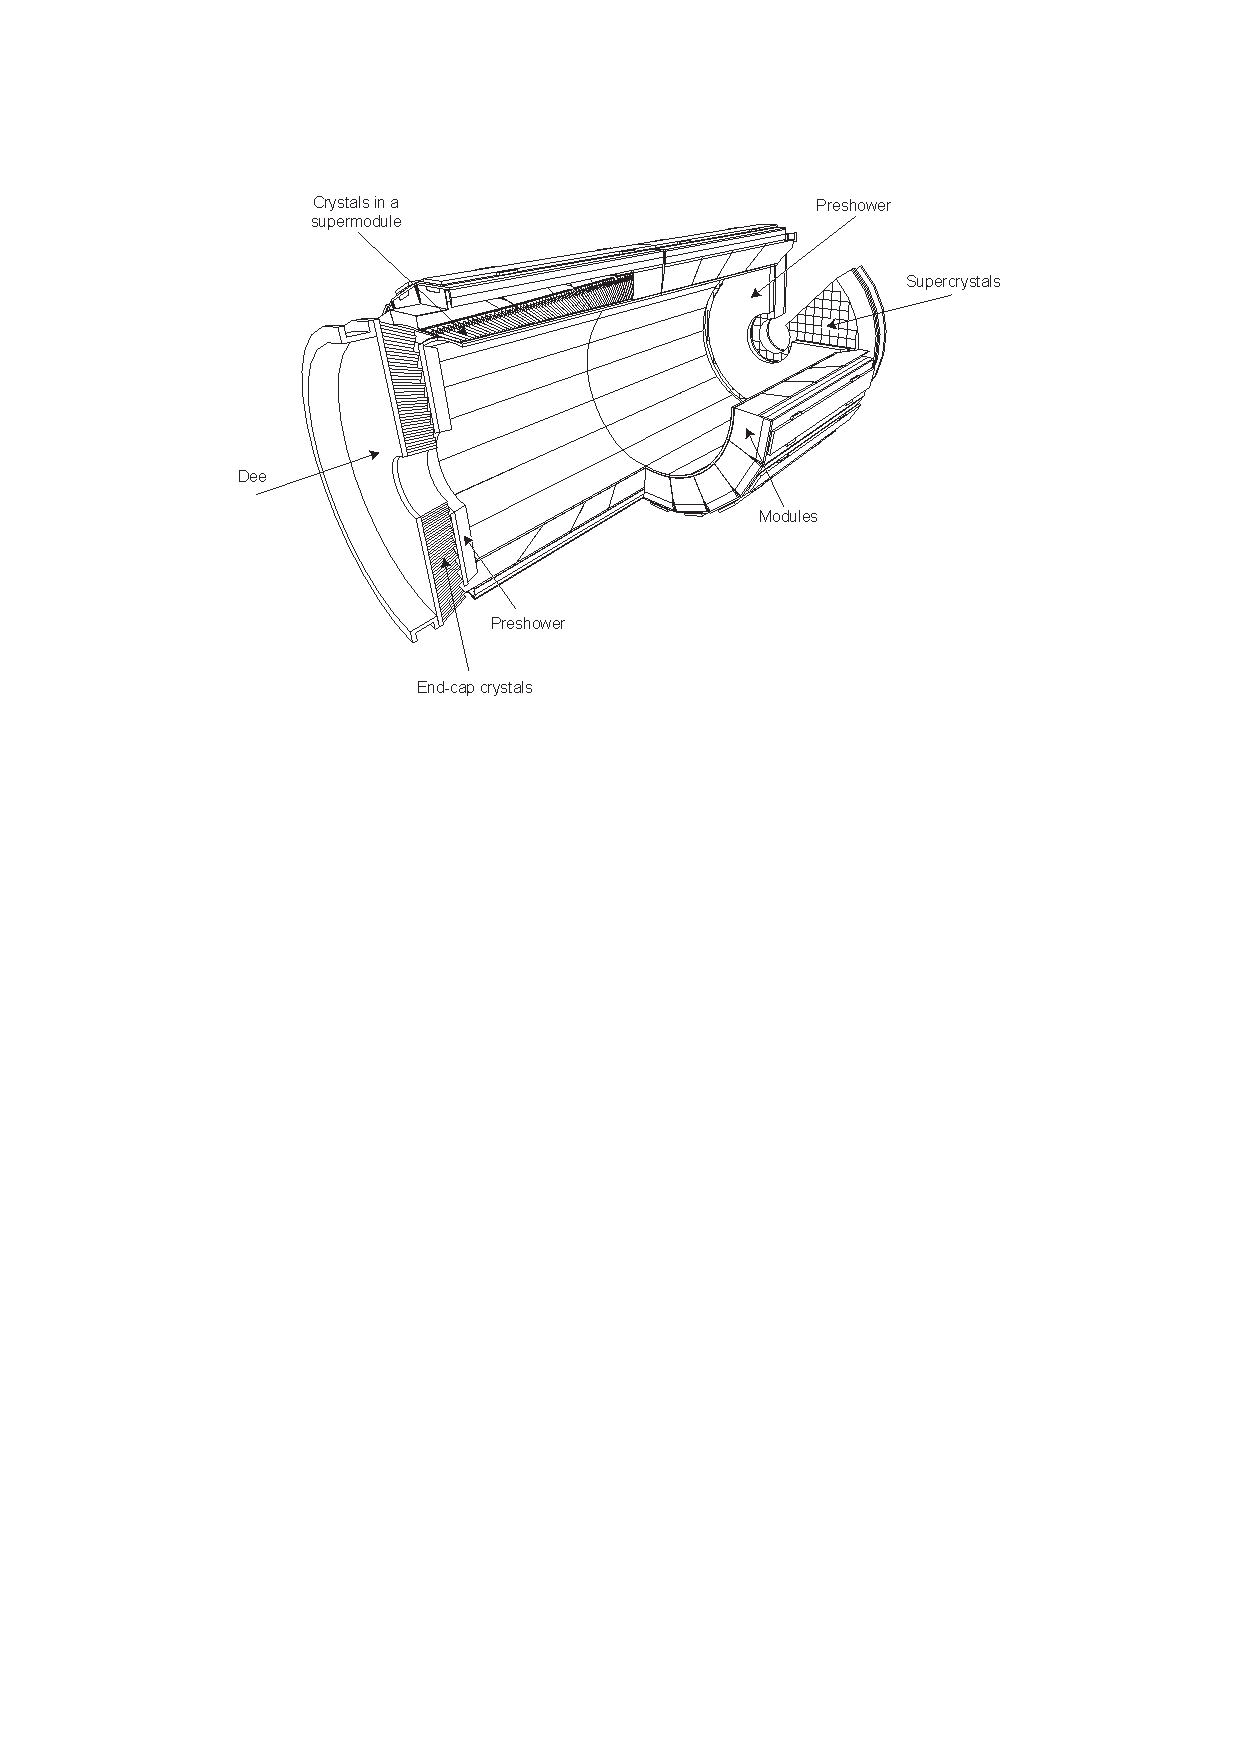
\includegraphics[width=0.8\textwidth]{Figures/ECAL.pdf}
		%\rule{35em}{0.5pt}
	\caption[CMS Electromagnetic Calorimeter]{A drawing of the CMS electromagnetic calorimeter. \cite{Chatrchyan:2008aa}}
	\label{fig:ECAL}
\end{figure}
\par Operation temperature of the detector is 18$\deg$C at which $\sim$4.5 photoelectrons are collected per MeV. The blue-green scintillation light is measured my the avalanche photodiodes in the barrel and vacuum phototriodes in the endcaps.   
\par The ECAL energy resolution is affected by three uncorrelated sources. Equation \ref{eq:ECAL_res} shows the parametrisation of the ECAL resolution where parameters $a$, $b$ and $c$ are determined from the test beam. The stohactic term $a$ is very low for the lead tungstate crystals ($a$ = 2.83$\pm$0.3$\%$) which means that showers can be mostly contained within the crystals. The noise term $b$ is determined from the electronics and is usually $b=124$ MeV. The last term $c$ is the constant term which limits the ECAL accuracy at high energies.   
\begin{equation}
\left(\frac{\sigma_E}{E}\right)^2 = \left(\frac{a}{\sqrt{E}}\right)^2 + \left(\frac{b}{E}\right)^2 + c^2
\label{eq:ECAL_res}
\end{equation}   

%----------------------------------------------------------------------------------------
%	SECTION 4
%----------------------------------------------------------------------------------------

\section{Hadronic calorimeter}

Hadronic calorimeter is used to measure energies of hadrons like pions, kaons, protons neutrons etc. Barrel and endcap hadronic calorimeters cover the pseudorapidity rande to $|\eta|=3$. 
Since in the transverse direction, the absorber thickness is only 5.82 interaction lengths, additional layer was placed outside the solenoid.  Hadronic calorimeter is a sampling calorimeter which consists of layers of brass and plastic scintillator layers. Showers are produced mostly in brass and are detected in the scintillator and reemitted in the narrow wavelength range in which photodetectors operate. In the endcap region, steel and quartz are used because of higher radiation hardness. There is an additional part of the detector placed 11.2 meters from the interaction point on both sides called forward HCAL which extends the coverage to $|\eta|=5.2$. Large HCAL coverage and good energy measurement are very important for jet reconstruction as well as for missing transverse energy measurement.  
\begin{figure}[htbp]
	\centering
		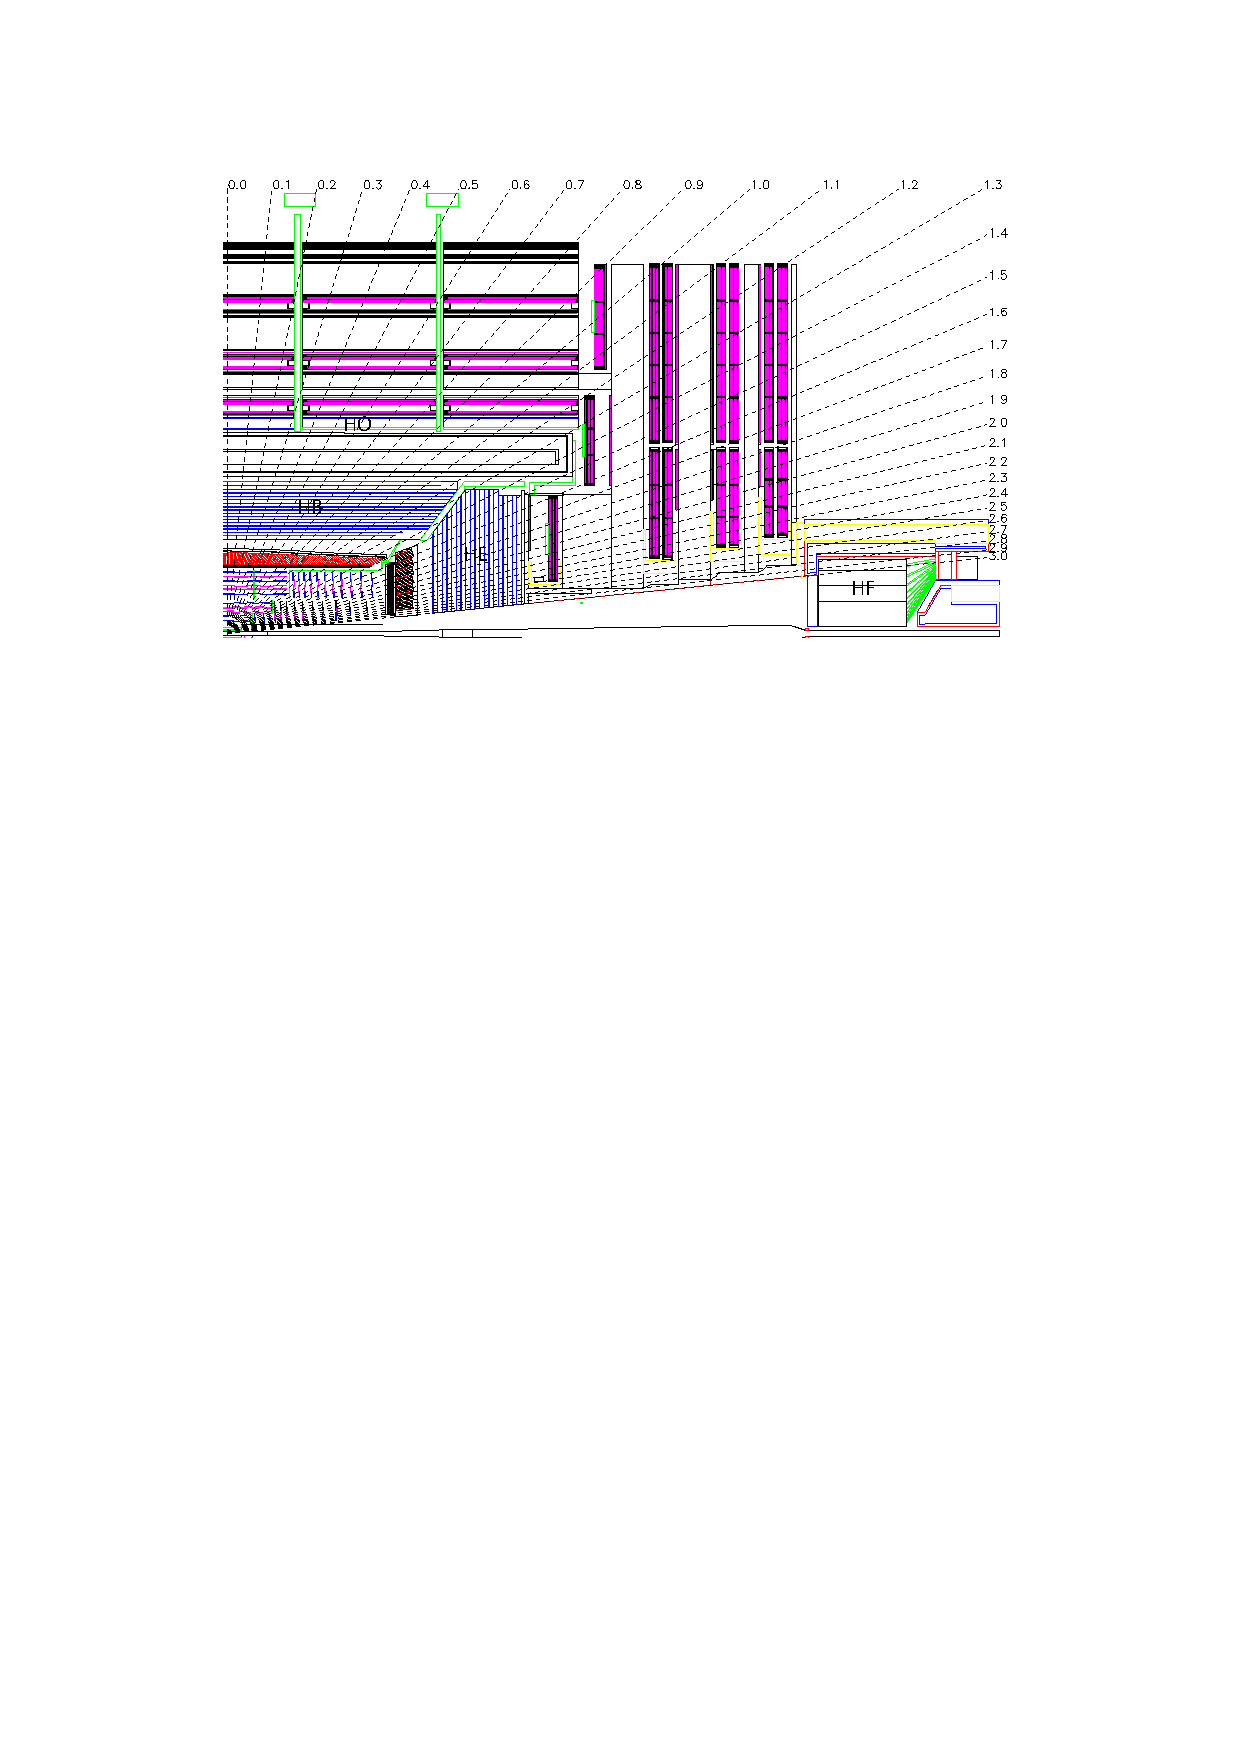
\includegraphics[width=0.8\textwidth]{Figures/HCAL.pdf}
		%\rule{35em}{0.5pt}
	\caption[CMS Hadronic Calorimeter]{A drawing of the CMS Hadronic Calorimeter. \cite{Chatrchyan:2008aa}}
	\label{fig:HCAL}
\end{figure}


%----------------------------------------------------------------------------------------
%	SECTION 5
%----------------------------------------------------------------------------------------

\section{Muon chambers}

Muons are the only particles that pass the calorimeters and the solenoid and their charge and momentum is measured again in the outer part of the detector by the muon chambers. There are three different types of the gaseous detectors used in the muon system, Drift tubes (DT), Resistive Plate Chambers (RPC) and Cathode Strip Chambers (CSC). Drift tubes are used in the barrel region where muon rate is relatively low and covers pseudorapidity range of $|\eta|<1.2$. The signal in Drift tubes is generated when a particle ionizes the gas inside the tube and the charge is collected by wires which are at high voltages. Cathode Strip chambers are used in the endcap region where muon rate is much higher and magnetic field is not uniform. These are multi-wire proportional chambers with anodes that collect charge from the gas ionization. Resistive Plate Chambers are placed both in barrel and endcap region. These detectors are designed as two parallel plates which create a uniform electric field in the gas between them. The electrodes on the plates are highly resistive so that when charged particle passes, it causes an electron avalanche which passes through the plates and is collected by the external metallic strips. Their time resolution is of the order $\sim$1 ns which makes RPCs a good choice for triggering although their spatial resolution is not so good.
\begin{figure}[htbp]
	\centering
		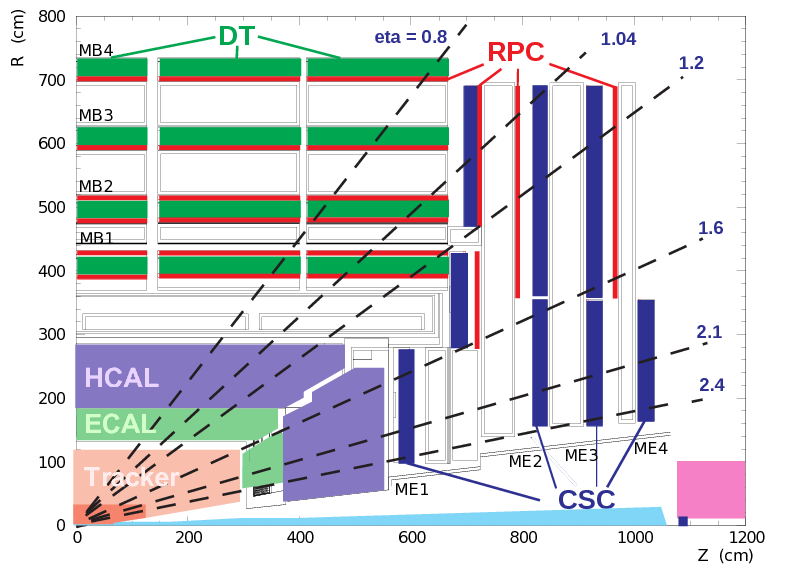
\includegraphics[width=0.8\textwidth]{Figures/Muon_chambres.png}
		%\rule{35em}{0.5pt}
	\caption[CMS Muon Chambers]{A drawing of the CMS muon chambers which consist of three different types of the detectors: DRift tubes, Cathode Strip Chambers and Resistive Plate chambers. \cite{Chatrchyan:2008aa}}
	\label{fig:Mu}
\end{figure} 
 
\par Large magnetic field enables even for high $p_T$ muons to be measured with a reasonable cell size in the muon chambers. The limiting factor for good resolution of low $p_T$ muons in multiple scattering, and for high $p_T$ muons the chamber resolution. The momentum resolution as a function of muon $p_T$ is shown in Figure \ref{fig:MU_pt} and it shows both muon chambers resolution and inner tracker resolution together with the combined result. 
\begin{figure}[htbp]
	\centering
		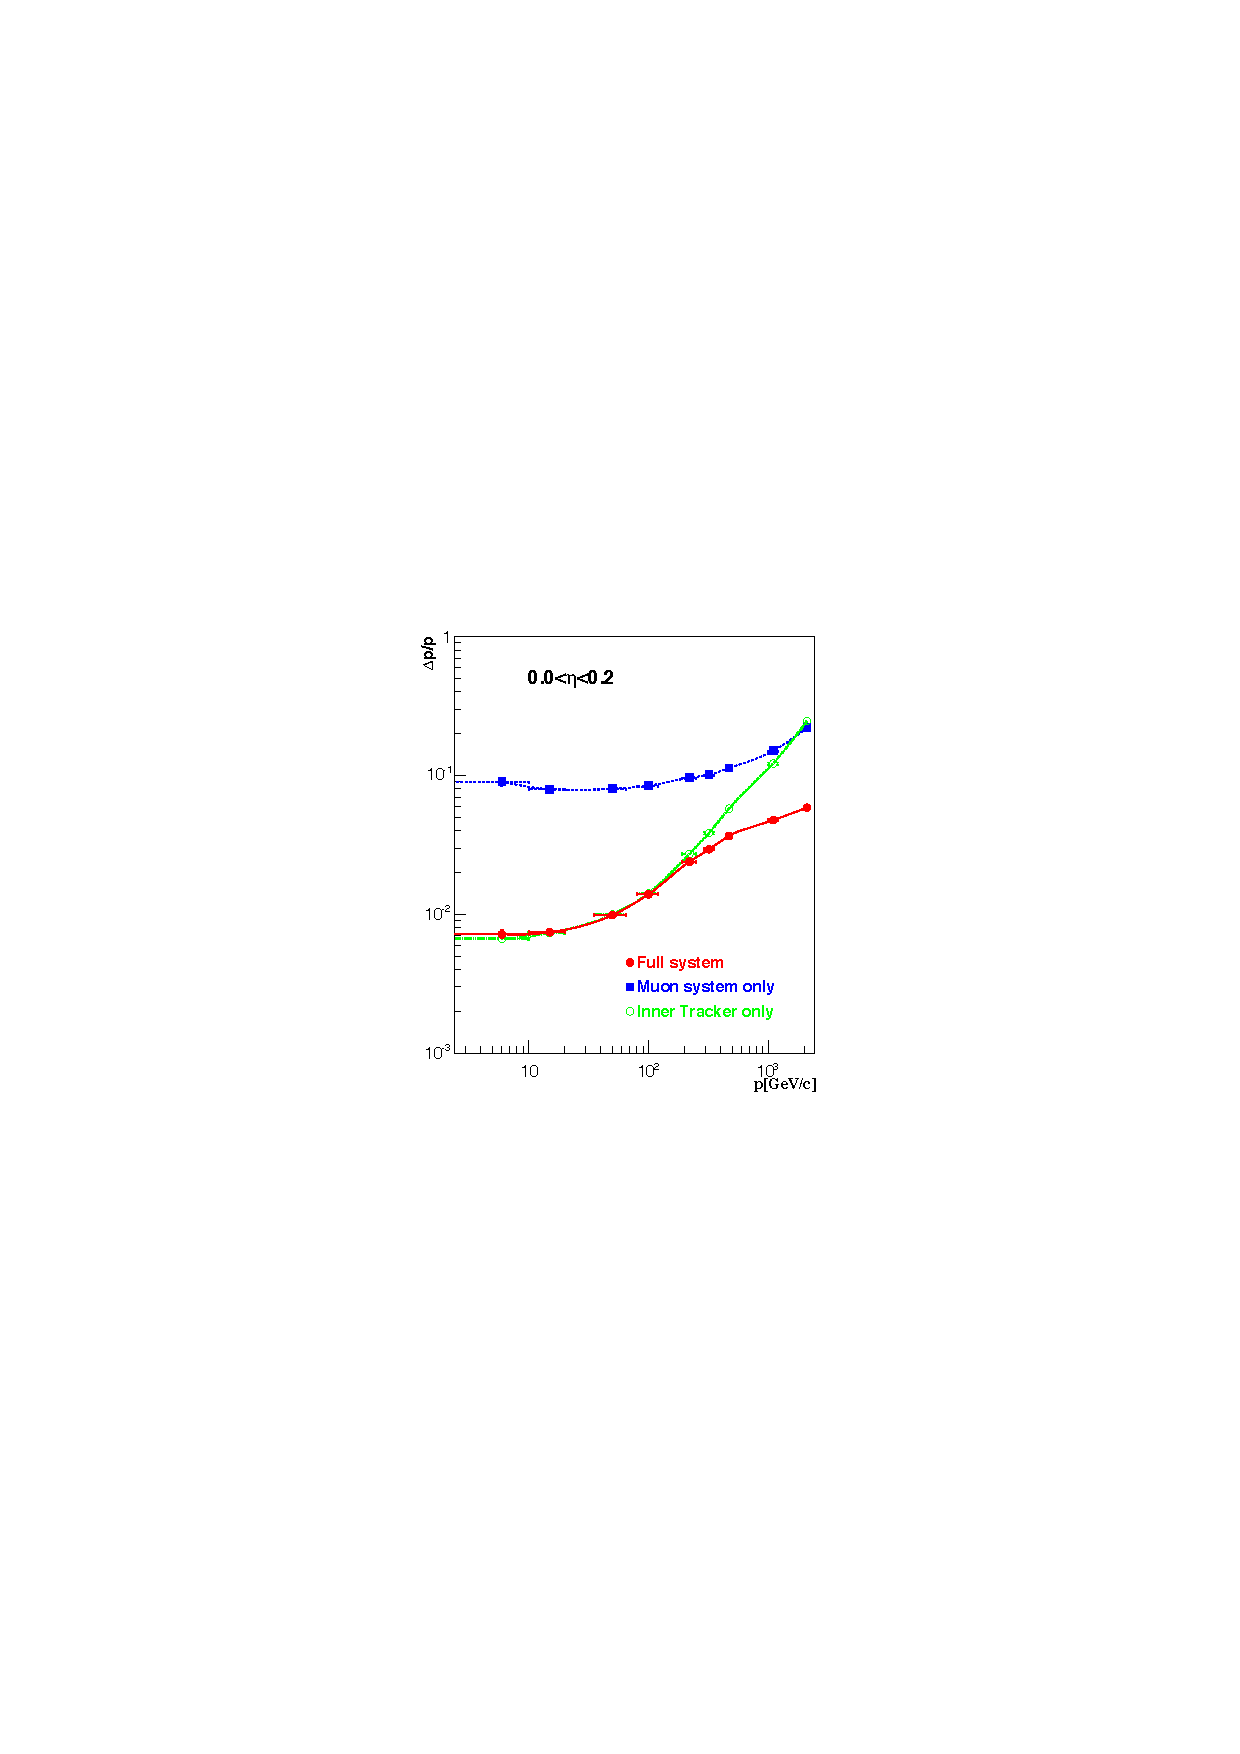
\includegraphics[width=0.5\textwidth]{Figures/MU_pt_res.pdf}
		%\rule{35em}{0.5pt}
	\caption[Muon resolution measurements for tracker, muon chambers and combined]{Muon resolution measurements for tracker, muon chambers and combined \cite{Chatrchyan:2008aa}}
	\label{fig:MU_pt}
\end{figure} 


%----------------------------------------------------------------------------------------
%	SECTION 6
%----------------------------------------------------------------------------------------

\section{Trigger}

The design rate of the proton collisions at the LHC is 40 MHz, although during Run 1 data taking period, the rate was 20 MHz which corresponds to 50 ns bunch spacing. Data from each of the bunch crossings is called an event. Since there are huge amounts of data coming from the subdetectors, it is necessary to apply some conditions which can reduce the rate to about 100 events per second. This is done by two level triggering system, first one called Level 1(L1) trigger and secong one called High Level Trigger(HLT). L1 trigger uses a special costum made electronics designed to reduce the output rate from 40 MHz to 100 kHz. Events which pass some loose criteria are than passed to the HLT. The L1 trigger uses the information from Calorimeters and Muon chambers to take the decision whether the event should be accepted or rejected usually searching fo presence of muons, jets above certain $p_T$, or looking at the total amount of $E_T$ and $E_T^{miss}$. The time needed to send the signals to the electronics, run the L1 selection and send the information back to the subdetectors in 3.2 $\mu$s. After L1 accepted the event, it is stored in the readout buffers where partial reconstruction takes place and the event is than processed by the HLT. This is a software farm which reduces the number of events to about 100 per second. 
\begin{figure}[htbp]
	\centering
		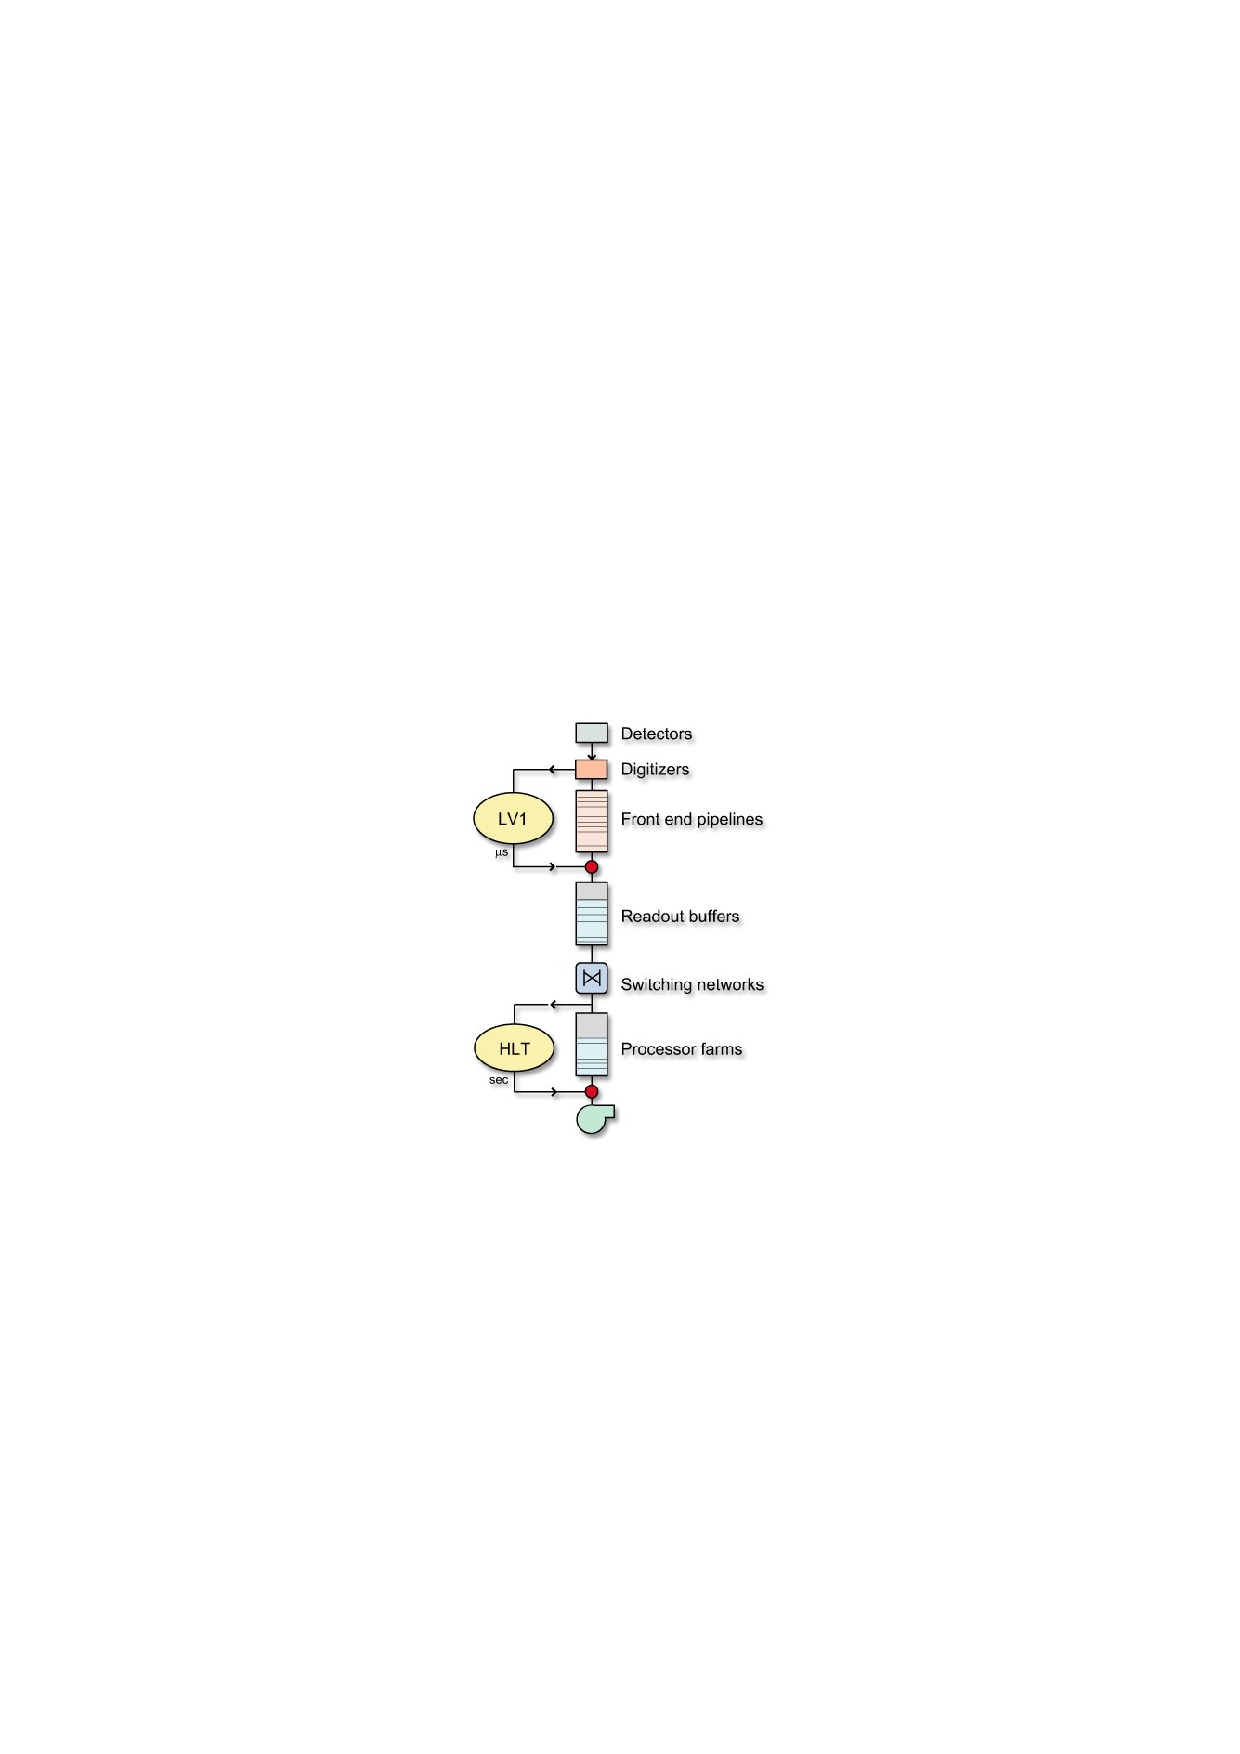
\includegraphics[width=0.5\textwidth]{Figures/trigger.pdf}
		%\rule{35em}{0.5pt}
	\caption[A drawing of CMS Trigger System.]{A drawing of CMS Trigger System. \cite{Chatrchyan:2008aa}}
	\label{fig:trig}
\end{figure}

